% One outcome of Kac's coins for the primes 2, 3, 5 and 7. Heads on 2 and 5, tails on 3 and 7.
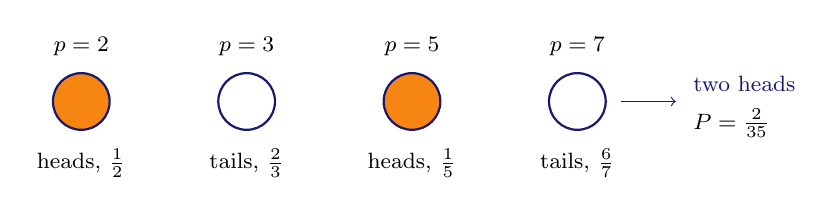
\begin{tikzpicture}[every node/.style={font=\footnotesize}]
  \fill[BurntOrange] (0,0) circle (0.36);
  \draw[MidnightBlue,thick] (0,0) circle (0.36);
  \node[above] at (0,0.46) {$p=2$};
  \node[below] at (0,-0.48) {heads, $\frac12$};

  \draw[MidnightBlue,thick] (2.1,0) circle (0.36);
  \node[above] at (2.1,0.46) {$p=3$};
  \node[below] at (2.1,-0.48) {tails, $\frac23$};

  \fill[BurntOrange] (4.2,0) circle (0.36);
  \draw[MidnightBlue,thick] (4.2,0) circle (0.36);
  \node[above] at (4.2,0.46) {$p=5$};
  \node[below] at (4.2,-0.48) {heads, $\frac15$};

  \draw[MidnightBlue,thick] (6.3,0) circle (0.36);
  \node[above] at (6.3,0.46) {$p=7$};
  \node[below] at (6.3,-0.48) {tails, $\frac67$};

  \draw[MidnightBlue,->] (6.85,0)--(7.55,0);
  \node[anchor=west,MidnightBlue] at (7.65,0.22) {two heads};
  \node[anchor=west] at (7.65,-0.28) {$P=\frac{2}{35}$};
\end{tikzpicture}
